\tab Vom adauga fisierele noi create pe repozitoriul nostru. Pentru aceasta vom avea nevoie de
urmatoarele comenzi :\\
\textbf{git add *} - comanda indexeaza toate fisierele.\\
\textbf{git commit -m} - comanda face un snapshot la toate schimbarile noastre.\\
\textbf{git push origin master} - comanda incarca toate fisierele indexate pe git.\\
\\
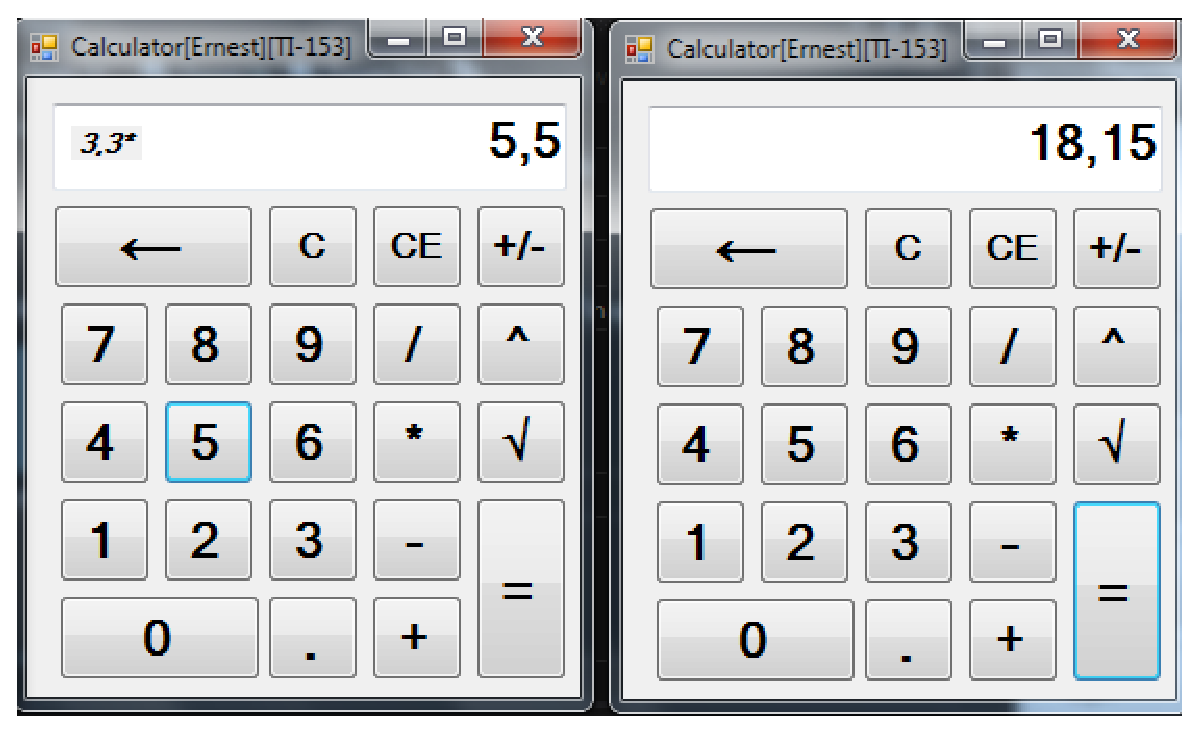
\includegraphics[width=\textwidth]{5.eps}
\\
\\
\tab Pentru a ne asigura ca am facut totul bine si nu avem probleme vom utiliza :\textbf{git status} si \textbf{git show}\\
\\
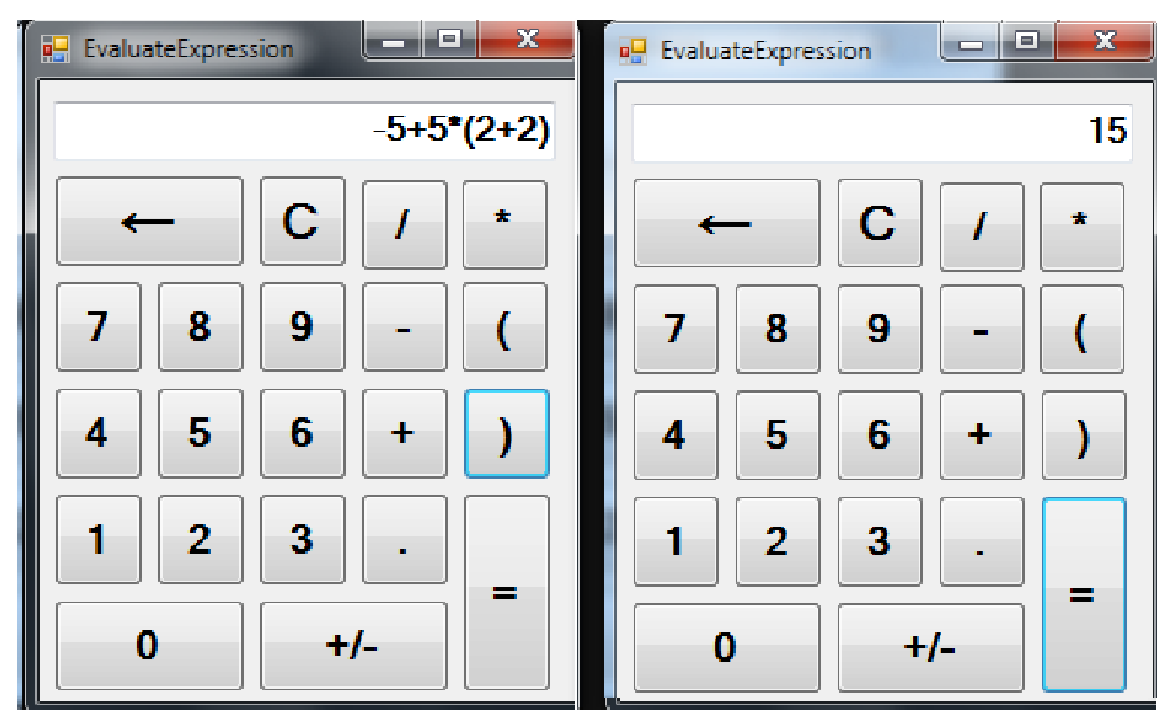
\includegraphics[width=\textwidth]{6.eps}
